% This file was created by matlab2tikz.
%
\documentclass[tikz]{standalone}
\usepackage[T1]{fontenc}
\usepackage[utf8]{inputenc}
\usepackage{pgfplots}
\usepackage{grffile}
\pgfplotsset{compat=newest}
\usetikzlibrary{plotmarks}
\usepgfplotslibrary{patchplots}
\usepackage{amsmath}

\newlength\figureHeight \setlength{\figureHeight}{6cm}
\newlength\figureWidth \setlength{\figureWidth}{10cm}
\begin{document}
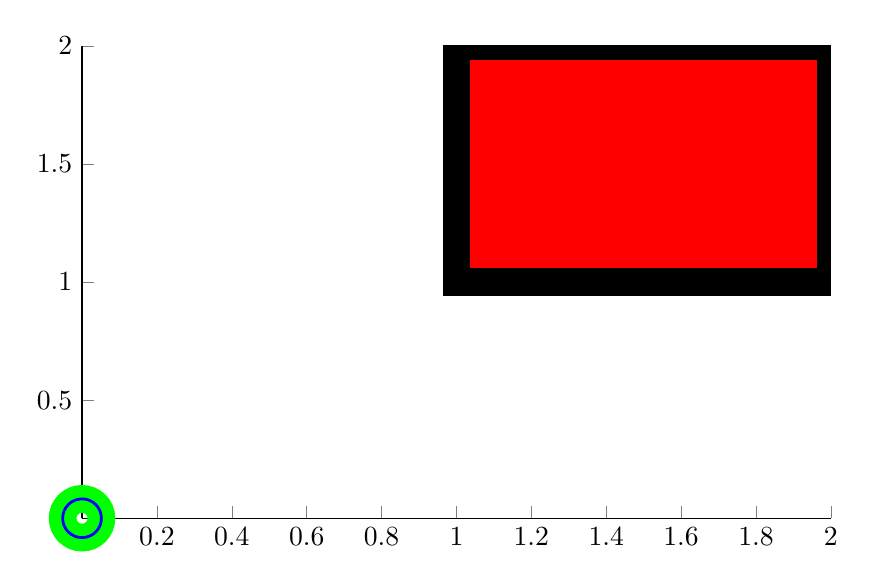
\begin{tikzpicture}

\begin{axis}[%
width=0.951\figureWidth,
height=\figureHeight,
at={(0\figureWidth,0\figureHeight)},
scale only axis,
xmin=   0,
xmax=   2,
ymin=   0,
ymax=   2,
axis background/.style={fill=white},
axis x line*=bottom,
axis y line*=left
]

\addplot[area legend,solid,line width=10.0pt,draw=black,fill=red,forget plot]
table[row sep=crcr] {%
x	y\\
   1	   1\\
   1	   2\\
   2	   2\\
   2	   1\\
}--cycle;
\addplot [color=green,line width=10.0pt,mark size=7.0pt,only marks,mark=o,mark options={solid},forget plot]
  table[row sep=crcr]{%
   0	   0\\
};
\addplot [color=blue,line width=1.0pt,mark size=7.0pt,only marks,mark=o,mark options={solid},forget plot]
  table[row sep=crcr]{%
   0	   0\\
};
\end{axis}
\end{tikzpicture}%
\end{document}